% Created by tikzDevice version 0.12.6 on 2024-07-30 18:39:29
% !TEX encoding = UTF-8 Unicode
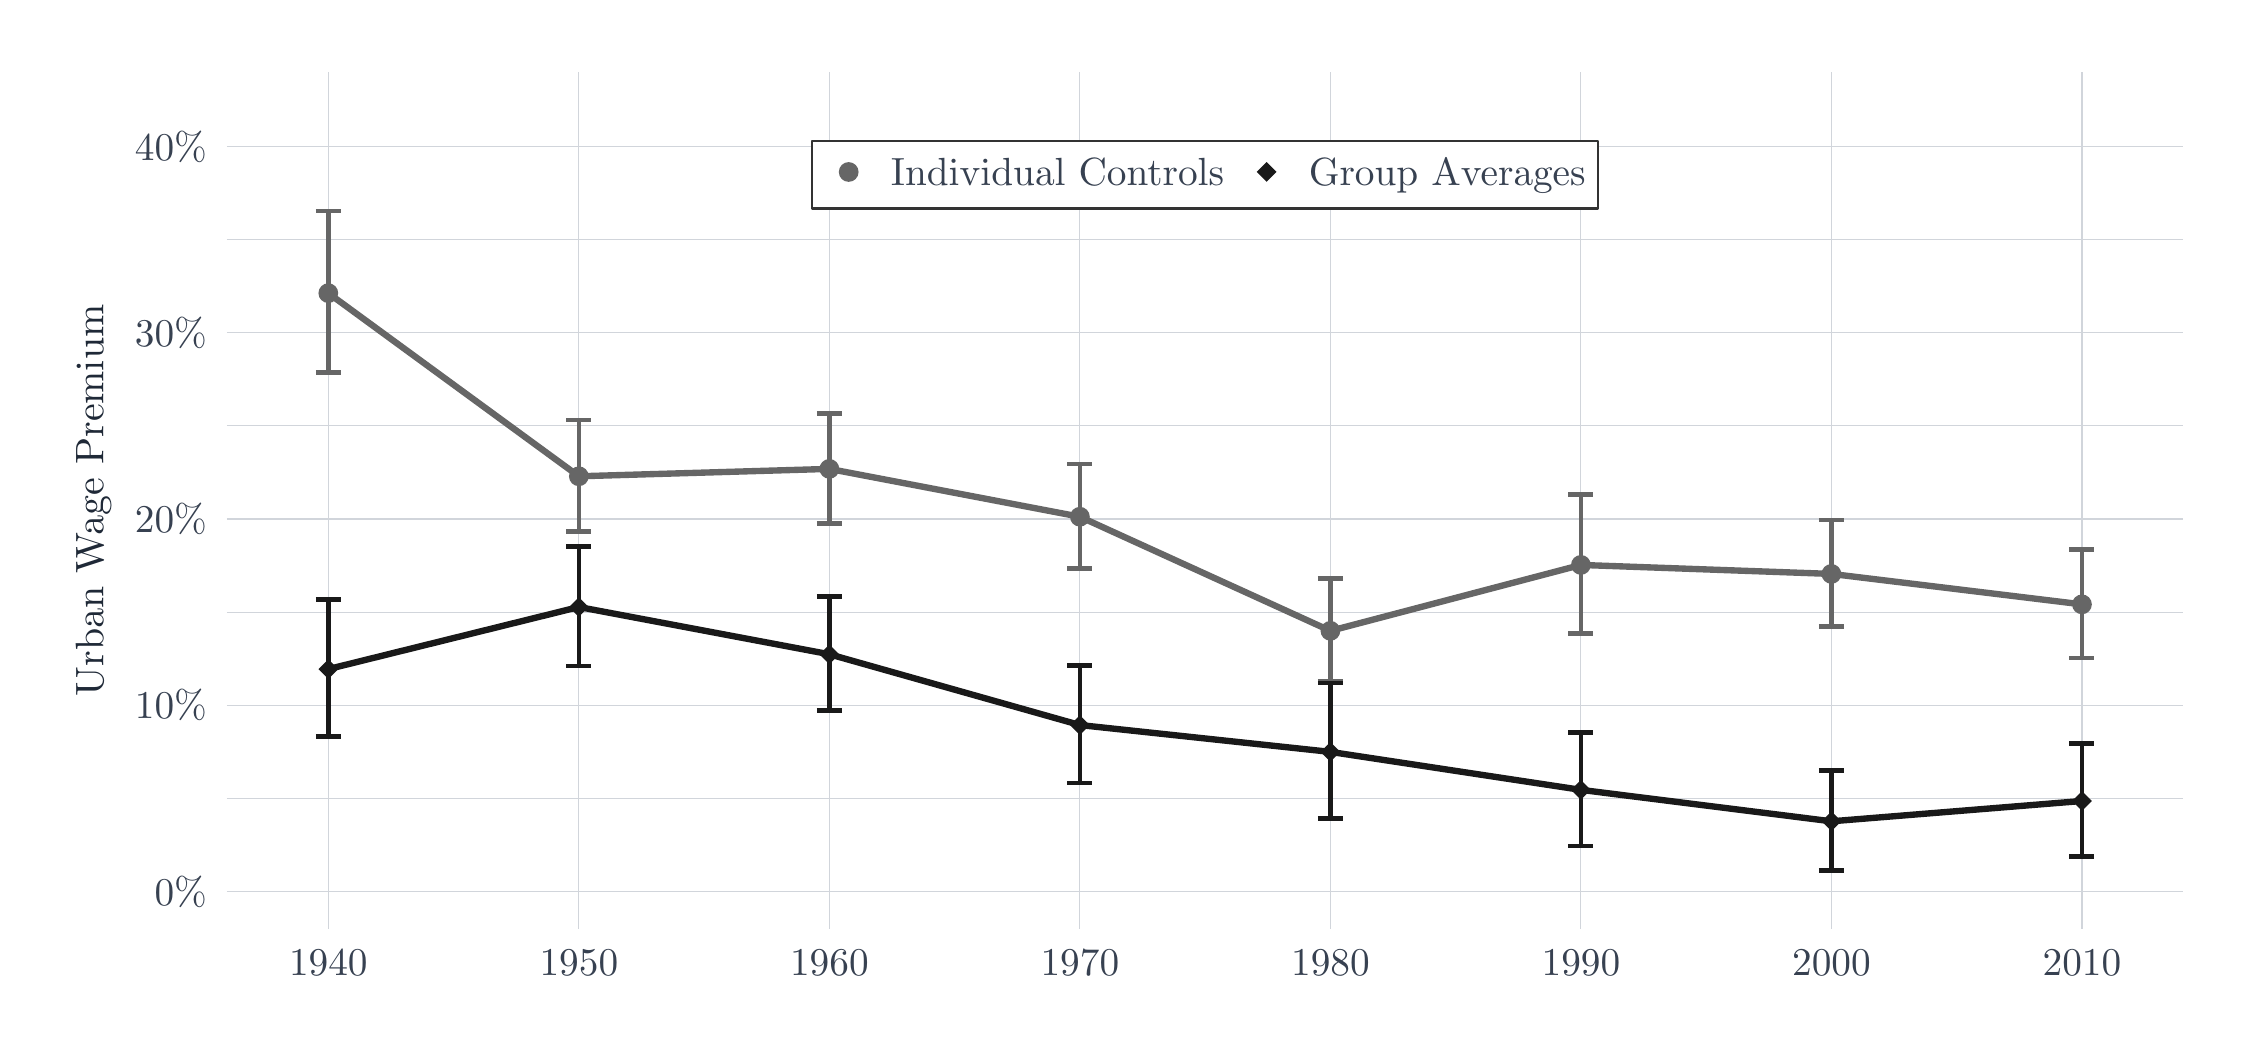
\begin{tikzpicture}[x=1pt,y=1pt]
\definecolor{fillColor}{RGB}{255,255,255}
\path[use as bounding box,fill=fillColor] (0,0) rectangle (794.97,361.35);
\begin{scope}
\path[clip] (  0.00,  0.00) rectangle (794.97,361.35);
\definecolor{drawColor}{RGB}{255,255,255}

\path[draw=drawColor,line width= 0.8pt,line join=round,line cap=round,fill=fillColor] (  0.00,  0.00) rectangle (794.97,361.35);
\end{scope}
\begin{scope}
\path[clip] ( 71.98, 35.76) rectangle (778.97,345.35);
\definecolor{drawColor}{RGB}{255,255,255}
\definecolor{fillColor}{RGB}{255,255,255}

\path[draw=drawColor,line width= 0.8pt,line join=round,line cap=round,fill=fillColor] ( 71.98, 35.76) rectangle (778.97,345.35);
\definecolor{drawColor}{RGB}{209,213,219}

\path[draw=drawColor,line width= 0.4pt,line join=round] ( 71.98, 82.87) --
	(778.97, 82.87);

\path[draw=drawColor,line width= 0.4pt,line join=round] ( 71.98,150.17) --
	(778.97,150.17);

\path[draw=drawColor,line width= 0.4pt,line join=round] ( 71.98,217.47) --
	(778.97,217.47);

\path[draw=drawColor,line width= 0.4pt,line join=round] ( 71.98,284.78) --
	(778.97,284.78);

\path[draw=drawColor,line width= 0.4pt,line join=round] ( 71.98, 49.22) --
	(778.97, 49.22);

\path[draw=drawColor,line width= 0.4pt,line join=round] ( 71.98,116.52) --
	(778.97,116.52);

\path[draw=drawColor,line width= 0.4pt,line join=round] ( 71.98,183.82) --
	(778.97,183.82);

\path[draw=drawColor,line width= 0.4pt,line join=round] ( 71.98,251.13) --
	(778.97,251.13);

\path[draw=drawColor,line width= 0.4pt,line join=round] ( 71.98,318.43) --
	(778.97,318.43);

\path[draw=drawColor,line width= 0.4pt,line join=round] (108.64, 35.76) --
	(108.64,345.35);

\path[draw=drawColor,line width= 0.4pt,line join=round] (199.17, 35.76) --
	(199.17,345.35);

\path[draw=drawColor,line width= 0.4pt,line join=round] (289.69, 35.76) --
	(289.69,345.35);

\path[draw=drawColor,line width= 0.4pt,line join=round] (380.21, 35.76) --
	(380.21,345.35);

\path[draw=drawColor,line width= 0.4pt,line join=round] (470.74, 35.76) --
	(470.74,345.35);

\path[draw=drawColor,line width= 0.4pt,line join=round] (561.26, 35.76) --
	(561.26,345.35);

\path[draw=drawColor,line width= 0.4pt,line join=round] (651.78, 35.76) --
	(651.78,345.35);

\path[draw=drawColor,line width= 0.4pt,line join=round] (742.31, 35.76) --
	(742.31,345.35);
\definecolor{drawColor}{gray}{0.40}

\path[draw=drawColor,line width= 2.3pt,line join=round] (108.64,265.42) --
	(199.17,199.24) --
	(289.69,201.91) --
	(380.21,184.62) --
	(470.74,143.39) --
	(561.26,167.21) --
	(651.78,163.96) --
	(742.31,152.96);
\definecolor{drawColor}{gray}{0.10}

\path[draw=drawColor,line width= 2.3pt,line join=round] (108.64,129.57) --
	(199.17,152.00) --
	(289.69,134.93) --
	(380.21,109.35) --
	(470.74, 99.65) --
	(561.26, 85.93) --
	(651.78, 74.57) --
	(742.31, 81.91);
\definecolor{drawColor}{gray}{0.40}

\path[draw=drawColor,line width= 1.7pt,line join=round] (104.12,295.09) --
	(113.17,295.09);

\path[draw=drawColor,line width= 1.7pt,line join=round] (108.64,295.09) --
	(108.64,236.71);

\path[draw=drawColor,line width= 1.7pt,line join=round] (104.12,236.71) --
	(113.17,236.71);
\definecolor{drawColor}{gray}{0.10}

\path[draw=drawColor,line width= 1.7pt,line join=round] (104.12,154.75) --
	(113.17,154.75);

\path[draw=drawColor,line width= 1.7pt,line join=round] (108.64,154.75) --
	(108.64,105.20);

\path[draw=drawColor,line width= 1.7pt,line join=round] (104.12,105.20) --
	(113.17,105.20);
\definecolor{drawColor}{gray}{0.40}

\path[draw=drawColor,line width= 1.7pt,line join=round] (194.64,219.61) --
	(203.69,219.61);

\path[draw=drawColor,line width= 1.7pt,line join=round] (199.17,219.61) --
	(199.17,179.37);

\path[draw=drawColor,line width= 1.7pt,line join=round] (194.64,179.37) --
	(203.69,179.37);
\definecolor{drawColor}{gray}{0.10}

\path[draw=drawColor,line width= 1.7pt,line join=round] (194.64,173.93) --
	(203.69,173.93);

\path[draw=drawColor,line width= 1.7pt,line join=round] (199.17,173.93) --
	(199.17,130.68);

\path[draw=drawColor,line width= 1.7pt,line join=round] (194.64,130.68) --
	(203.69,130.68);
\definecolor{drawColor}{gray}{0.40}

\path[draw=drawColor,line width= 1.7pt,line join=round] (285.16,222.04) --
	(294.22,222.04);

\path[draw=drawColor,line width= 1.7pt,line join=round] (289.69,222.04) --
	(289.69,182.27);

\path[draw=drawColor,line width= 1.7pt,line join=round] (285.16,182.27) --
	(294.22,182.27);
\definecolor{drawColor}{gray}{0.10}

\path[draw=drawColor,line width= 1.7pt,line join=round] (285.16,155.80) --
	(294.22,155.80);

\path[draw=drawColor,line width= 1.7pt,line join=round] (289.69,155.80) --
	(289.69,114.62);

\path[draw=drawColor,line width= 1.7pt,line join=round] (285.16,114.62) --
	(294.22,114.62);
\definecolor{drawColor}{gray}{0.40}

\path[draw=drawColor,line width= 1.7pt,line join=round] (375.69,203.65) --
	(384.74,203.65);

\path[draw=drawColor,line width= 1.7pt,line join=round] (380.21,203.65) --
	(380.21,166.04);

\path[draw=drawColor,line width= 1.7pt,line join=round] (375.69,166.04) --
	(384.74,166.04);
\definecolor{drawColor}{gray}{0.10}

\path[draw=drawColor,line width= 1.7pt,line join=round] (375.69,130.94) --
	(384.74,130.94);

\path[draw=drawColor,line width= 1.7pt,line join=round] (380.21,130.94) --
	(380.21, 88.37);

\path[draw=drawColor,line width= 1.7pt,line join=round] (375.69, 88.37) --
	(384.74, 88.37);
\definecolor{drawColor}{gray}{0.40}

\path[draw=drawColor,line width= 1.7pt,line join=round] (466.21,162.25) --
	(475.26,162.25);

\path[draw=drawColor,line width= 1.7pt,line join=round] (470.74,162.25) --
	(470.74,124.98);

\path[draw=drawColor,line width= 1.7pt,line join=round] (466.21,124.98) --
	(475.26,124.98);
\definecolor{drawColor}{gray}{0.10}

\path[draw=drawColor,line width= 1.7pt,line join=round] (466.21,124.53) --
	(475.26,124.53);

\path[draw=drawColor,line width= 1.7pt,line join=round] (470.74,124.53) --
	(470.74, 75.60);

\path[draw=drawColor,line width= 1.7pt,line join=round] (466.21, 75.60) --
	(475.26, 75.60);
\definecolor{drawColor}{gray}{0.40}

\path[draw=drawColor,line width= 1.7pt,line join=round] (556.73,192.78) --
	(565.79,192.78);

\path[draw=drawColor,line width= 1.7pt,line join=round] (561.26,192.78) --
	(561.26,142.43);

\path[draw=drawColor,line width= 1.7pt,line join=round] (556.73,142.43) --
	(565.79,142.43);
\definecolor{drawColor}{gray}{0.10}

\path[draw=drawColor,line width= 1.7pt,line join=round] (556.73,106.78) --
	(565.79,106.78);

\path[draw=drawColor,line width= 1.7pt,line join=round] (561.26,106.78) --
	(561.26, 65.68);

\path[draw=drawColor,line width= 1.7pt,line join=round] (556.73, 65.68) --
	(565.79, 65.68);
\definecolor{drawColor}{gray}{0.40}

\path[draw=drawColor,line width= 1.7pt,line join=round] (647.26,183.46) --
	(656.31,183.46);

\path[draw=drawColor,line width= 1.7pt,line join=round] (651.78,183.46) --
	(651.78,144.92);

\path[draw=drawColor,line width= 1.7pt,line join=round] (647.26,144.92) --
	(656.31,144.92);
\definecolor{drawColor}{gray}{0.10}

\path[draw=drawColor,line width= 1.7pt,line join=round] (647.26, 92.93) --
	(656.31, 92.93);

\path[draw=drawColor,line width= 1.7pt,line join=round] (651.78, 92.93) --
	(651.78, 56.68);

\path[draw=drawColor,line width= 1.7pt,line join=round] (647.26, 56.68) --
	(656.31, 56.68);
\definecolor{drawColor}{gray}{0.40}

\path[draw=drawColor,line width= 1.7pt,line join=round] (737.78,172.80) --
	(746.83,172.80);

\path[draw=drawColor,line width= 1.7pt,line join=round] (742.31,172.80) --
	(742.31,133.61);

\path[draw=drawColor,line width= 1.7pt,line join=round] (737.78,133.61) --
	(746.83,133.61);
\definecolor{drawColor}{gray}{0.10}

\path[draw=drawColor,line width= 1.7pt,line join=round] (737.78,102.69) --
	(746.83,102.69);

\path[draw=drawColor,line width= 1.7pt,line join=round] (742.31,102.69) --
	(742.31, 61.73);

\path[draw=drawColor,line width= 1.7pt,line join=round] (737.78, 61.73) --
	(746.83, 61.73);
\definecolor{fillColor}{gray}{0.40}

\path[fill=fillColor] (108.64,265.42) circle (  3.57);
\definecolor{fillColor}{gray}{0.10}

\path[fill=fillColor] (105.07,129.57) --
	(108.64,133.14) --
	(112.21,129.57) --
	(108.64,126.00) --
	cycle;
\definecolor{fillColor}{gray}{0.40}

\path[fill=fillColor] (199.17,199.24) circle (  3.57);
\definecolor{fillColor}{gray}{0.10}

\path[fill=fillColor] (195.60,152.00) --
	(199.17,155.57) --
	(202.73,152.00) --
	(199.17,148.44) --
	cycle;
\definecolor{fillColor}{gray}{0.40}

\path[fill=fillColor] (289.69,201.91) circle (  3.57);
\definecolor{fillColor}{gray}{0.10}

\path[fill=fillColor] (286.12,134.93) --
	(289.69,138.50) --
	(293.26,134.93) --
	(289.69,131.36) --
	cycle;
\definecolor{fillColor}{gray}{0.40}

\path[fill=fillColor] (380.21,184.62) circle (  3.57);
\definecolor{fillColor}{gray}{0.10}

\path[fill=fillColor] (376.64,109.35) --
	(380.21,112.92) --
	(383.78,109.35) --
	(380.21,105.78) --
	cycle;
\definecolor{fillColor}{gray}{0.40}

\path[fill=fillColor] (470.74,143.39) circle (  3.57);
\definecolor{fillColor}{gray}{0.10}

\path[fill=fillColor] (467.17, 99.65) --
	(470.74,103.22) --
	(474.31, 99.65) --
	(470.74, 96.08) --
	cycle;
\definecolor{fillColor}{gray}{0.40}

\path[fill=fillColor] (561.26,167.21) circle (  3.57);
\definecolor{fillColor}{gray}{0.10}

\path[fill=fillColor] (557.69, 85.93) --
	(561.26, 89.50) --
	(564.83, 85.93) --
	(561.26, 82.36) --
	cycle;
\definecolor{fillColor}{gray}{0.40}

\path[fill=fillColor] (651.78,163.96) circle (  3.57);
\definecolor{fillColor}{gray}{0.10}

\path[fill=fillColor] (648.22, 74.57) --
	(651.78, 78.14) --
	(655.35, 74.57) --
	(651.78, 71.00) --
	cycle;
\definecolor{fillColor}{gray}{0.40}

\path[fill=fillColor] (742.31,152.96) circle (  3.57);
\definecolor{fillColor}{gray}{0.10}

\path[fill=fillColor] (738.74, 81.91) --
	(742.31, 85.48) --
	(745.88, 81.91) --
	(742.31, 78.34) --
	cycle;
\end{scope}
\begin{scope}
\path[clip] (  0.00,  0.00) rectangle (794.97,361.35);
\definecolor{drawColor}{RGB}{55,65,81}

\node[text=drawColor,anchor=base east,inner sep=0pt, outer sep=0pt, scale=  1.42] at ( 64.78, 44.32) {0\%};

\node[text=drawColor,anchor=base east,inner sep=0pt, outer sep=0pt, scale=  1.42] at ( 64.78,111.62) {10\%};

\node[text=drawColor,anchor=base east,inner sep=0pt, outer sep=0pt, scale=  1.42] at ( 64.78,178.93) {20\%};

\node[text=drawColor,anchor=base east,inner sep=0pt, outer sep=0pt, scale=  1.42] at ( 64.78,246.23) {30\%};

\node[text=drawColor,anchor=base east,inner sep=0pt, outer sep=0pt, scale=  1.42] at ( 64.78,313.53) {40\%};
\end{scope}
\begin{scope}
\path[clip] (  0.00,  0.00) rectangle (794.97,361.35);
\definecolor{drawColor}{RGB}{55,65,81}

\node[text=drawColor,anchor=base,inner sep=0pt, outer sep=0pt, scale=  1.42] at (108.64, 18.76) {1940};

\node[text=drawColor,anchor=base,inner sep=0pt, outer sep=0pt, scale=  1.42] at (199.17, 18.76) {1950};

\node[text=drawColor,anchor=base,inner sep=0pt, outer sep=0pt, scale=  1.42] at (289.69, 18.76) {1960};

\node[text=drawColor,anchor=base,inner sep=0pt, outer sep=0pt, scale=  1.42] at (380.21, 18.76) {1970};

\node[text=drawColor,anchor=base,inner sep=0pt, outer sep=0pt, scale=  1.42] at (470.74, 18.76) {1980};

\node[text=drawColor,anchor=base,inner sep=0pt, outer sep=0pt, scale=  1.42] at (561.26, 18.76) {1990};

\node[text=drawColor,anchor=base,inner sep=0pt, outer sep=0pt, scale=  1.42] at (651.78, 18.76) {2000};

\node[text=drawColor,anchor=base,inner sep=0pt, outer sep=0pt, scale=  1.42] at (742.31, 18.76) {2010};
\end{scope}
\begin{scope}
\path[clip] (  0.00,  0.00) rectangle (794.97,361.35);
\definecolor{drawColor}{RGB}{31,41,55}

\node[text=drawColor,rotate= 90.00,anchor=base,inner sep=0pt, outer sep=0pt, scale=  1.44] at ( 27.32,190.55) {Urban Wage Premium};
\end{scope}
\begin{scope}
\path[clip] (  0.00,  0.00) rectangle (794.97,361.35);
\definecolor{drawColor}{gray}{0.20}
\definecolor{fillColor}{RGB}{255,255,255}

\path[draw=drawColor,line width= 0.8pt,line join=round,line cap=round,fill=fillColor] (283.45,295.97) rectangle (567.50,320.43);
\end{scope}
\begin{scope}
\path[clip] (  0.00,  0.00) rectangle (794.97,361.35);
\definecolor{drawColor}{RGB}{255,255,255}
\definecolor{fillColor}{RGB}{255,255,255}

\path[draw=drawColor,line width= 0.8pt,line join=round,line cap=round,fill=fillColor] (289.45,301.97) rectangle (303.90,316.43);
\end{scope}
\begin{scope}
\path[clip] (  0.00,  0.00) rectangle (794.97,361.35);
\definecolor{fillColor}{gray}{0.40}

\path[fill=fillColor] (296.67,309.20) circle (  3.57);
\end{scope}
\begin{scope}
\path[clip] (  0.00,  0.00) rectangle (794.97,361.35);
\definecolor{drawColor}{RGB}{255,255,255}
\definecolor{fillColor}{RGB}{255,255,255}

\path[draw=drawColor,line width= 0.8pt,line join=round,line cap=round,fill=fillColor] (440.46,301.97) rectangle (454.92,316.43);
\end{scope}
\begin{scope}
\path[clip] (  0.00,  0.00) rectangle (794.97,361.35);
\definecolor{fillColor}{gray}{0.10}

\path[fill=fillColor] (444.12,309.20) --
	(447.69,312.77) --
	(451.26,309.20) --
	(447.69,305.63) --
	cycle;
\end{scope}
\begin{scope}
\path[clip] (  0.00,  0.00) rectangle (794.97,361.35);
\definecolor{drawColor}{RGB}{55,65,81}

\node[text=drawColor,anchor=base west,inner sep=0pt, outer sep=0pt, scale=  1.42] at (311.90,304.30) {Individual Controls};
\end{scope}
\begin{scope}
\path[clip] (  0.00,  0.00) rectangle (794.97,361.35);
\definecolor{drawColor}{RGB}{55,65,81}

\node[text=drawColor,anchor=base west,inner sep=0pt, outer sep=0pt, scale=  1.42] at (462.92,304.30) {Group Averages};
\end{scope}
\end{tikzpicture}
